\chapter{Matching and Assignment Problem}

Ajur and Jura were startled to hear the footsteps behind them. They turned back and saw Rishnak standing. Rishnak said the edges analog of maximal independent set (set of non-adjacent vertices) is a maximal matching. Maximal matching is a set of edges that do not share any common end vertices. Rishnak showed a graph Figure \ref{16g1} and the maximal matching edges are colored red.
\begin{figure}
\begin{center}

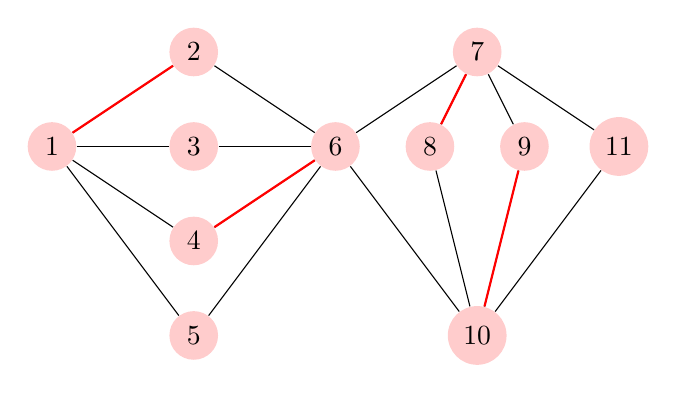
\begin{tikzpicture}
  [scale=.6,auto=left,every node/.style={circle,fill=red!20}]
  \node (n1) at (-1,1) {1};
  \node (n2) at (2,3)  {2};
  \node (n3) at (2,1)  {3};
  \node (n4) at (2,-1) {4};
  \node (n5) at (2, -3) {5};
  \node (n6) at (5,1)  {6};
  \node (n7) at (8,3)  {7};
  \node (n8) at (7,1) {8};
  \node (n9) at (9,1)  {9};
  \node (n10) at (8,-3)  {10};
  \node (n11) at (11,1) {11};

  \foreach \from/\to in {n1/n2,n1/n3,n1/n4,n1/n5,n2/n6,n3/n6/n4,n4/n6,n5/n6,n6/n7,n6/n10,n7/n8,n7/n9,n7/n11,
  n8/n10,n9/n10,n10/n11}
    \draw (\from) -- (\to);
\draw[-,thick,red]
  (n1) to (n2);
  \draw[-,thick,red]
  (n4) to (n6);
  \draw[-,thick,red]
  (n7) to (n8);
  \draw[-,thick,red]
  (n9) to (n10);
  \end{tikzpicture}
\caption{Maximal Matching edges in this graph are colored red}\label{16g1}
\end{center}
\end{figure}

Since this is a maximal matching - every edge is incident at one of the end vertices of the edges in the Maximal set. Hence the vertices $\{1,2,4,6,7,8,9,10\}$ form a vertex cover. However the minimum vertex cover is $\{1,6,7,10\}$. If we find a Maximal matching we know the bound on the size of the minimum vertex cover!.
